\documentclass[11pt,oneside]{article}
\usepackage[T1]{fontenc}
\usepackage[utf8]{inputenc}
%\DeclareUnicodeCharacter{00A0}{ }
\usepackage[adobe-utopia]{mathdesign}

\usepackage{amsmath}
\usepackage[francais]{babel}
\usepackage[dvips]{graphicx}
%\usepackage{here}
\usepackage{framed}
\usepackage[normalem]{ulem}
\usepackage{fancyhdr}
\usepackage{titlesec}
\usepackage{vmargin}

\usepackage{amsmath}
\usepackage{ifthen}
\usepackage{multirow}
\usepackage{multicol} % Portions de texte en colonnes

%\usepackage{xltxtra} % Logo XeLaTeX
%\usepackage{pst-solides3d}
\usepackage{color}
%\usepackage{colortbl}
\usepackage{titletoc} % Pour la mise en forme de la table des matières

%\usepackage[crop=off]{auto-pst-pdf}
%\usepackage{bclogo}


%\usepackage{longtable}
%\usepackage{flafter}%floatants après la référence
%\usepackage{pst-solides3d}
%\usepackage{pstricks}
%\usepackage{minitoc}
%\setcounter{minitocdepth}{4}
%\usepackage{draftcopy}% "Brouillon"
%\usepackage{floatflt}
%\usepackage{psfrag}
%\usepackage{listings} % Permet d'insérer du code de programmation
%\usepackage{lmodern}
%\usepackage[adobe-utopia,uppercase=upright,greeklowercase=upright]{mathdesign}
%\usepackage{minionpro}
%\usepackage{pifont}
%\usepackage{amssymb}
%\usepackage[francais]{varioref}

\setmarginsrb{1.5cm}{1cm}{1cm}{1.5cm}{1cm}{1cm}{1cm}{1cm}

\definecolor{gris25}{gray}{0.75}
\definecolor{bleu}{RGB}{18,33,98}
\definecolor{bleuf}{RGB}{42,94,171}
\definecolor{bleuc}{RGB}{231,239,247}
\definecolor{rougef}{RGB}{185,18,27}
\definecolor{rougec}{RGB}{255,230,231}
\definecolor{vertf}{RGB}{103,126,82}
\definecolor{vertc}{RGB}{220,255,191}
\definecolor{violetf}{RGB}{112,48,160}
\definecolor{violetc}{RGB}{230,224,236}
\definecolor{jaunec}{RGB}{220,255,191}
\usepackage[final]{pdfpages} 
\usepackage[%
    pdftitle={TD Conception},
    pdfauthor={Xavier Pessoles},
    colorlinks=true,
    linkcolor=blue,
    citecolor=magenta]{hyperref}



% \makeatletter \let\ps@plain\ps@empty \makeatother
%% DEBUT DU DOCUMENT
%% =================
\sloppy
\hyphenpenalty 10000

\newcommand{\Pointilles}[1][3]{%
\multido{}{#1}{\makebox[\linewidth]{\dotfill}\\[\parskip]
}}


\begin{document}


\newboolean{prof}
\setboolean{prof}{false}
%------------- En tetes et Pieds de Pages ------------
\pagestyle{fancy}
\renewcommand{\headrulewidth}{0pt}

\fancyhead{}
\fancyhead[L]{%
\begin{minipage}[c]{1.6cm}

\includegraphics[width=2cm]{png/logo_ptsi.png}%
\end{minipage}
\rule{2cm}{.5pt}
}

\fancyhead[C]{\rule{11cm}{.5pt}}

\fancyhead[R]{%
\begin{minipage}[c]{3cm}
\begin{flushright}
\footnotesize{\textit{\textsf{Sciences Industrielles\\ pour l'Ingénieur}}}%
\end{flushright}
\end{minipage}
}

\renewcommand{\footrulewidth}{0.2pt}

\fancyfoot[C]{\footnotesize{\bfseries \thepage}}
\fancyfoot[L]{\footnotesize{2012 -- 2013} \\ X. \textsc{Pessoles}}
\ifthenelse{\boolean{prof}}{%
\fancyfoot[R]{\footnotesize{TD -- CI 4 -- Conception des mécanismes -- P}}
}{%
\fancyfoot[R]{\footnotesize{TD -- CI 4 -- Conception des mécanismes}}
}


%\begin{center}
%\textit{Centre d'intérêt}
%\end{center}


\begin{center}
 \Large\textsc{CI 4 -- Conception des mécanismes}
\end{center}


\begin{center}
 \large\textsc{Tendeur de courroie}
\end{center}
\vspace{.5cm}

\begin{flushright}
\textit{D'après ressources de Jean-Pierre Pupier.}
\end{flushright}

\begin{contexte}
\begin{itemize}
\item Objectif pédagogique : concevoir un système mécanique
\item Objectif technique : 
\begin{itemize}
\item Proposer une solution technologique permettant de concevoir un tendeur de courroie
\end{itemize}
\end{itemize}
\end{contexte}


\subsection*{Description}

Le mécanisme représente un dispositif pour tendre une courroie de transmission d’une machine. 

\begin{minipage}[c]{.3\linewidth}
\begin{center}
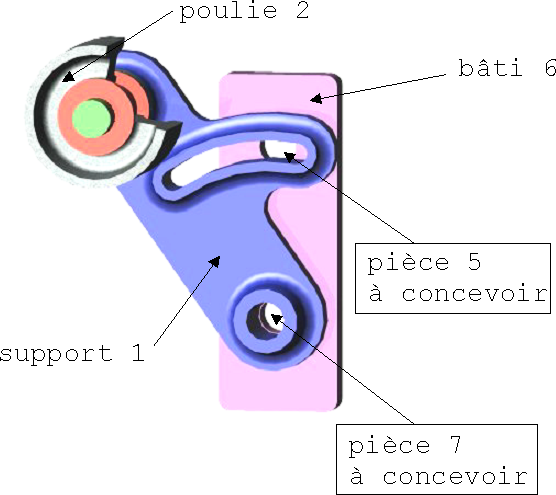
\includegraphics[height=4cm]{png/fig1}

\end{center}
\end{minipage}\hfill
\begin{minipage}[c]{.3\linewidth}
\begin{center}
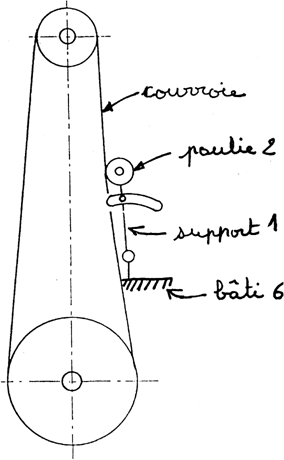
\includegraphics[height=4cm]{png/fig2}

\end{center}
\end{minipage}\hfill
\begin{minipage}[c]{.3\linewidth}
\begin{center}
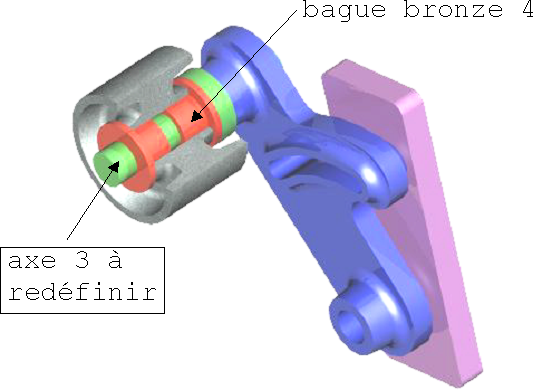
\includegraphics[height=4cm]{png/fig3}

\end{center}
\end{minipage}

\vspace{.5cm}

Il comprend un bâti fixe 6 sur lequel est monté un support 1 supportant la 
poulie 2.

Ce support peut être réglé par pivotement pour assurer la tension de la courroie.

\subsection*{Propositions de construction}
Il faudra donc s’attacher aux points suivants :
\begin{itemize}
\item le support 1 est en liaison pivot avec un axe 7 lié à 6 par une liaison encastrement démontable;
\item la position réglable du support 1 est fixée par un élément fileté 5 à concevoir. L’amplitude du réglage doit être de $45\degres$;
\item la poulie est munie d’une bague en bronze 4. Elle est en liaison pivot avec un axe 3;
\item l’axe 3 est lié à 1 par une liaison encastrement démontable;
\item le support 1 vient de fonderie au sable.
\end{itemize}

\subsection*{Travail à faire}
\paragraph{}
\textit{Traduisez sous forme de schéma cinématique les propositions de construction.}

\paragraph{}
\textit{Complétez la coupe AA montrant l’ensemble monté.}

\paragraph{}
\textit{Indiquez les ajustements en vous contentant de préciser s’ils sont « libres » ou « serrés ».}

\end{document}